\chapter{Étude statistique des algorithmes de résolution}\label{annexe_stats}
Le module \texttt{bn\_stats.py} fournit, dans la classe \texttt{Stats}, les outils pour analyser statistiquement une distribution de valeurs (calculs des indicateurs statistiques classiques, représentation en histogramme et diagramme en boîte grâce aux modules \texttt{numpy} et \texttt{matplotlib}).

Cette classe fournit également les outils pour sauvegarder et charger la liste des résultats bruts dans un fichier texte pour des analyses plus poussées futures.

Chaque graphique fait apparaître, outre l'histogramme de distribution des fréquences, les indicateurs suivants :
\begin{itemize}
\item moyenne et écart-type,
\item minimum, $Q_1$, médiane, $Q_3$ et maximum dans le diagramme en boîte,
\item le mode, noté à la base de la barre correspondante,
\item le temps moyen de résolution.
\end{itemize}

\medskip

La méthode de test est la suivante : on crée une liste \texttt{distrib} de longueur \texttt{xmax*ymax+1} qui est initialisée avec des valeurs nulles.\\
On répète $n$ fois la résolution sur une grille aléatoire, chaque fois différente et, en notant $k$ le nombre de coups de la résolution, on incrémente \texttt{distrib[k]} de 1.

\medskip

Le calcul du temps se fait en lançant un chronomètre grâce à la fonction \texttt{time()} du module \texttt{time}, qui renvoie le nombre de seconde écoulées depuis epoch (le 1\up{er} janvier 1970). Donc en sauvegardant cette valeur au début de la simulation dans une variable \texttt{start} et en calculant \texttt{time()-start} à la fin de la simulation, on obtient le temps total écoulé. Afin de chronométrer uniquement le temps de résolution (et non de la création de la grille), ce chronomètre est mis à jour uniquement lors de la résolution effective.

L'algorithme de test affiche une estimation du temps restant (ainsi que la date et l'heure de la fin de la simulation), ainsi que l'avancement par tranches de 10\%.

Afin d'obtenir des résultats comparables, tous les temps ont été mesurés sur le même ordinateur disposant d'un processeur Intel i7-4800-MQ cadencé à 2,7 GHz en mode monoprocesseur, de 16 Go de mémoire vive et tournant sous un système Linux 64 bits (Xubuntu 14.04).

\vfill 
\begin{flushright}
Résultats à partir de la page suivante $\rightarrow$
\end{flushright}
\newpage
\section{Niveau 1}
Dans ce niveau tous les tirs sont aléatoires uniformément sur les cases vides, et il n'y a pas de phase de tirs ciblés.\\
On obtient les résultats suivants sur un échantillon de $n=100\,000$ parties :

\begin{center}
\fbox{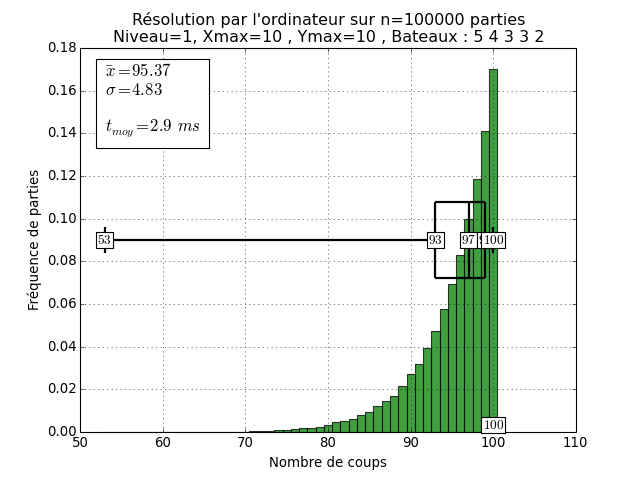
\includegraphics[scale=0.7]{./media/distrib_HAL_niveau=1_n=100000.png}}
\end{center}

Comme on pouvait s'y attendre, les résultats sont catastrophiques. Par contre la résolution est quasi immédiate (3 ms par partie en moyenne)
\newpage
\section{Niveau 2}
Au niveau 2, la phase de tirs en aveugle est aléatoire uniformément sur les cases vide, mais on ajoute la phase de tirs ciblés lorsqu'on touche un bateau.

Les résultats sur $n=100\,000$ parties sont les suivants :

\begin{center}
\fbox{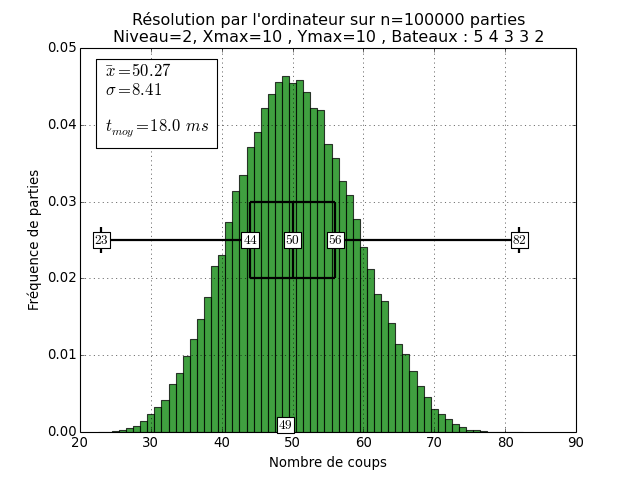
\includegraphics[scale=0.7]{./media/distrib_HAL_niveau=2_n=100000.png}}
\end{center}

Le fait de gérer la phase de tirs ciblés change radicalement les résultats. La forme de la courbe de distribution est d'ailleurs totalement différente de la précédente.\\
Par contre la résolutions prend 6 fois plus de temps.
\newpage
\section{Niveau 3}
Au niveau 3, la phase de tirs en aveugle est encore aléatoire mais uniquement sur les cases noires.

Les résultats sur $n=100\,000$ parties sont les suivants :

\begin{center}
\fbox{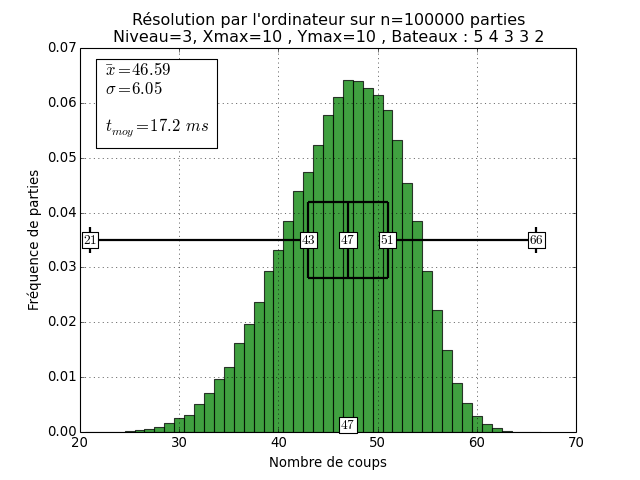
\includegraphics[scale=0.7]{./media/distrib_HAL_niveau=3_n=100000.png}}
\end{center}

On note une amélioration significative des performances, sans pour autant sacrifier en temps de résolution, au contraire puisqu'il faut moins de coups en aveugle pour finir la grille. Les résultats sont également plus homogènes ($\sigma=6,05$ au lieu de $8,41$ précédemment).

\newpage
\section{Niveau 4}
Au niveau 4 la détermination de la case optimale durant la phase de tirs en aveugle se fait en regardant, à chaque coup, un échantillon de taille \texttt{nb\_echantillons} de distributions de bateau aléatoires.

La valeur de \texttt{nb\_echantillons} va jouer sur les performances en nombre de coups (plus on fait d'échantillons et plus la distribution de probabilités obtenue est conforme à la vraie distribution de probabilité) mais aussi sur le temps de résolution. En effet ce dernier sera linéaire en \texttt{nb\_echantillons}.

Vu le temps de calcul, les simulations suivantes portent sur un nombre plus faible de parties (la contrainte fixée est que le calcul ne doit pas durer plus d'une nuit).
\subsection{Échantillons de taille \texttt{nb\_echantillons=10}}
Avec des échantillons de taille 10 nous obtenons les résultats suivants sur $n=10\,000$ parties :

\begin{center}
\fbox{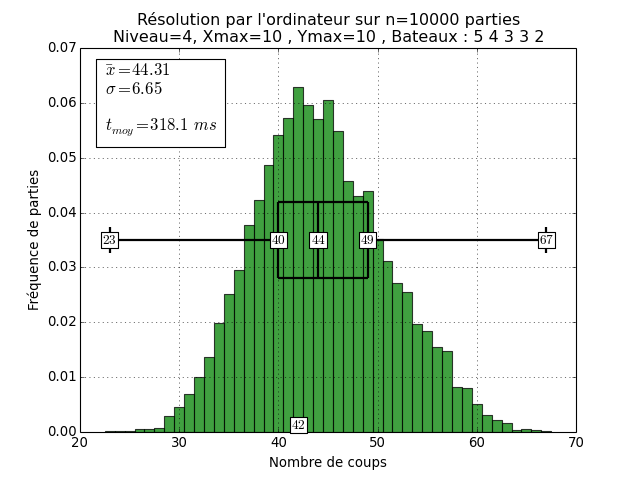
\includegraphics[scale=0.7]{./media/distrib_HAL_niveau=4(10)_n=10000.png}}
\end{center}

Avec une taille modeste des échantillons, nous obtenons une nette amélioration des performances avec une moyenne de 44,31,  pour un temps moyen de 0,3 secondes par partie.
 
\newpage
\subsection{Échantillons de taille \texttt{nb\_echantillons=100}}
Avec des échantillons de taille 100 nous obtenons les résultats suivants sur $n=10\,000$ parties :

\begin{center}
\fbox{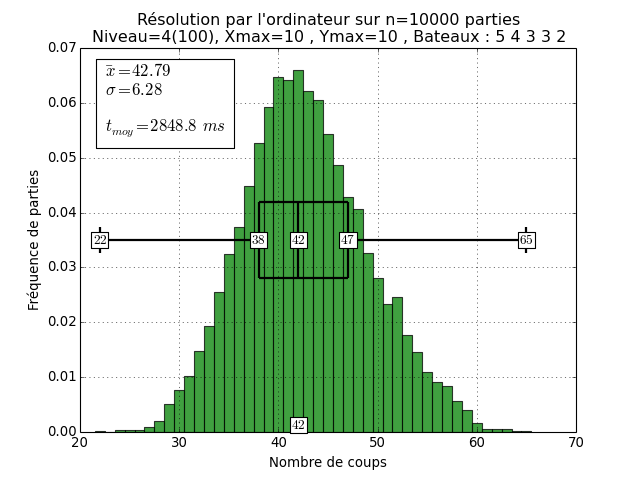
\includegraphics[scale=0.7]{./media/distrib_HAL_niveau=4(100)_n=10000.png}}
\end{center}
 
Les résultats sont très bons, avec une moyenne de 42,79 coups par partie, mais le temps de calcul commence à devenir long (presque 3 secondes par partie). 
 
\newpage
\section{Niveau 5}
Les résultats obtenues sur un échantillon de $n=1\,000\,000$ parties sont les suivants :
\begin{comment}
\begin{center}
\begin{tabular}[t]{|c|l|}
\hline
Nombre de coups & Effectifs\\
\hline
21 & 5\\
\hline
22 & 12\\
\hline
23 & 38\\
\hline
24 & 139\\
\hline
25 & 345\\
\hline
26 & 756\\
\hline
27 & 1635\\
\hline
28 & 3141\\
\hline
29 & 5188\\
\hline
30 & 8244\\
\hline
31 & 12579\\
\hline
32 & 17849\\
\hline
33 & 24091\\
\hline
34 & 30884\\
\hline
35 & 38162\\
\hline
36 & 45397\\
\hline
37 & 51988\\
\hline
38 & 57489\\
\hline
39 & 61778\\
\hline
40 & 64082\\
\hline
41 & 64215\\
\hline
42 & 62822\\
\hline
43 & 59966\\
\hline
\end{tabular}\hspace{0.5cm}
\begin{tabular}[t]{|c|l|}
\hline
Nombre de coups & Effectifs\\
\hline
44 & 56471\\
\hline
45 & 51981\\
\hline
46 & 46666\\
\hline
47 & 41422\\
\hline
48 & 35961\\
\hline
49 & 31474\\
\hline
50 & 26963\\
\hline
51 & 22700\\
\hline
52 & 19270\\
\hline
53 & 15816\\
\hline
54 & 12374\\
\hline
55 & 9586\\
\hline
56 & 6861\\
\hline
57 & 4819\\
\hline
58 & 3020\\
\hline
59 & 1844\\
\hline
60 & 1062\\
\hline
61 & 521\\
\hline
62 & 241\\
\hline
63 & 101\\
\hline
64 & 28\\
\hline
65 & 10\\
\hline
66 & 4\\
\hline
\end{tabular}
\end{center}
\end{comment}
\begin{center}
\fbox{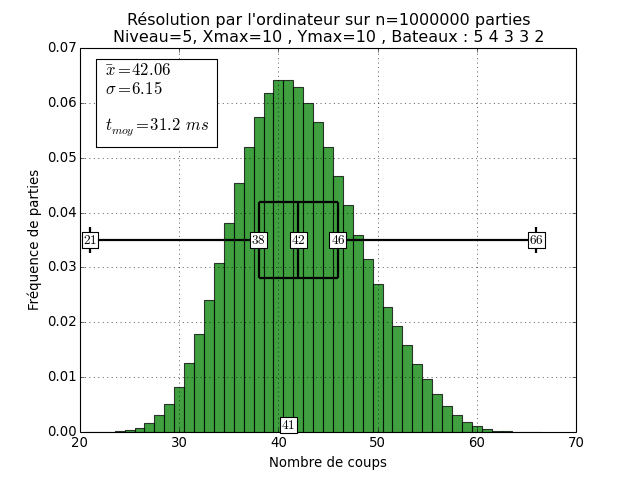
\includegraphics[scale=0.7]{./media/distrib_HAL_niveau=5_n=1000000.png}}
\end{center}

Notons les excellentes performances avec une moyenne de 42,06 coups pour un temps de résolution moyen de seulement 31,2 ms par partie.
